\section{Architectures}
See \cref{fig:Imp_Sty}

\begin{figure}
	\begin{center}
		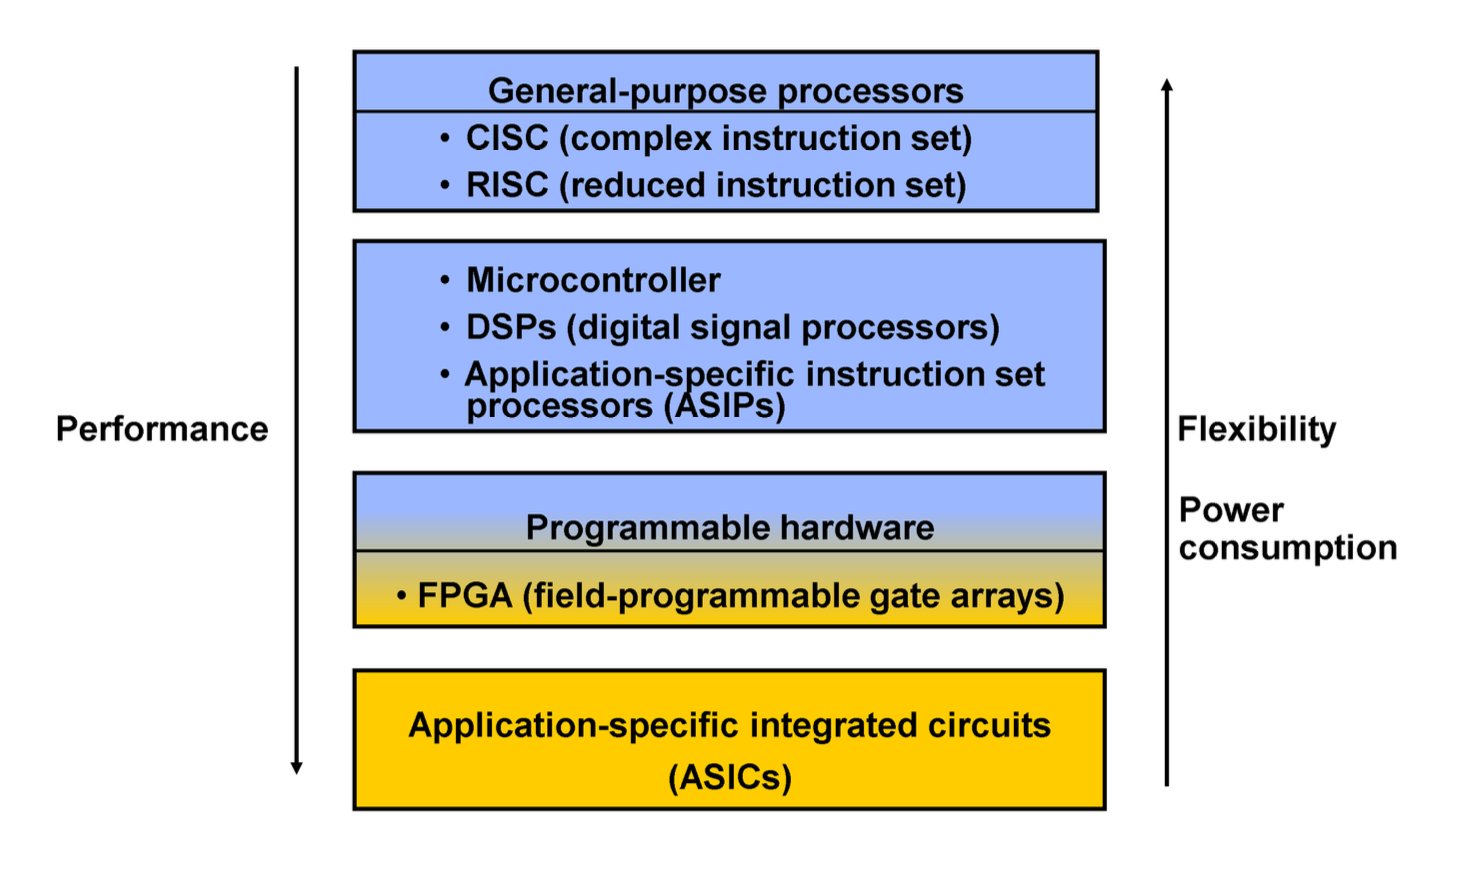
\includegraphics[width=0.5\textwidth]{images/Implementaion_styles.png}
		\caption{Implementation Styles}
		\label{fig:Imp_Sty}
	\end{center}
\end{figure}

\subsection{General-Purpose Processors}
\begin{itemize}
	\item Properties
		\begin{itemize}
			\item high performance for a broad range of applications, not optimized for any particular application
			\item high power consumption
		\end{itemize}
	\item Design
		\begin{itemize}
			\item highly optimized circuits
			\item design times > 100 person years
			\item cost/device only cheap when fabricated in huge numbers 
		\end{itemize}
	\item Application areas
		\begin{itemize}
			\item PCs
			\item Smartphones
		\end{itemize}
\end{itemize}

\subsubsection{Reasons for High Performance}
\begin{itemize}
	\item Exploitation of parallelism
		\begin{itemize}
			\item multiple scalar units (superscalar)
				\begin{itemize}
					\item Functional units: integer units, floating-point unit, load/store-unit
					\item Dynamic scheduling
					\item instruction compatibility
					\item complex control unit 
				\end{itemize}
			\item deep instruction pipeline
				\begin{itemize}
					\item fetch $\vert$ decode $\vert$ read $\vert$ execute $\vert$ write back
					\item each scalar unit my have individual pipeline depth
					\item branch prediction 
				\end{itemize}
		\end{itemize}
	\item Multi-level memory hierarchy 
		\begin{itemize}
			\item $\uparrow$ Speed $\Rightarrow$ $\downarrow$ Size $\Leftrightarrow$ $\uparrow$ Size $\Rightarrow$ $\downarrow$ Speed
			\item Register $<$ Cache $<$ Main Memory
		\end{itemize}
\end{itemize}

\subsubsection{General-Purpose Processors and Real-Time}
\begin{itemize}
	\item Execution time of programs is not well predictable 
		\begin{itemize}
			\item Dynamic scheduling
			\item Caching
			\item Branch prediction
		\end{itemize}
	\item Complex I/O and memory interface
\end{itemize}

\subsubsection{Multimedia - Extensions and Sub-words}
\begin{itemize}
	\item Multimedia Applications
		\begin{itemize}
			\item 8 / 16 Bit data types
			\item many arithmetic operations
			\item huge data sets $\Rightarrow$ Huge I/O-bandwidth
			\item high data parallelism 
		\end{itemize}
	\item Sub-word execution
		\begin{itemize}
			\item split 32/64-bit registers and ALUs into smaller sub-units
			\item instructions execute in parallel on these sub-units
			\item compromise between usage of parallelism and available data paths
			\item currently most often based on hand-written assembly routines
			\item Depends on language with defined bit width per data type and diverse overflow semantics
			\item Compiler needs to automatically detect sub-word parallelism 
		\end{itemize}
\end{itemize}

\subsection{Microcontrollers}
\begin{itemize}
	\item For control-dominant applications
		\begin{itemize}
			\item control flow dominant programs (many branches and jumps)
			\item few arithmetic operations
			\item low throughput requirements
			\item multitasking
		\end{itemize} 
	\item Microcontrollers are optimized for
		\begin{itemize}
			\item Bit- and logic-level operations
			\item Registers often realized in RAM: context switch through pointer operation, therefore shortest interrupt latencies
			\item integrated peripheral units (e.g. A/D, D/A, CAN, Timer)
		\end{itemize}
	\item Systems with 4/8 bit processors
	\item Microcontrollers with high performance
		\begin{itemize}
			\item 16 - 64 bit processors
			\item Application areas
				\begin{itemize}
					\item Systems with high control-dominant parts and additional demand
					\item High throughput (telecommunication, automotive)
					\item Computational power (industrial control, signal processing)
					\item As a part of an SOC
				\end{itemize}	
		\end{itemize}
\end{itemize}

\subsection{Digital Signal Processors}
\begin{itemize}
	\item Signal processing applications
	\begin{itemize}
		\item data-flow dominant
		\item many arithmetic operations, less branches and jumps
		\item high degree of parallelism
		\item high throughput requirements
	\end{itemize}
	\item DSPs are optimized for
	\begin{itemize}
		\item parallel instruction processing (MAC \cref{fig:MAC})
		\item Harvard Architecture, simultaneous access of multiple operands
		\item zero-overhead loops
		\item special addressing modes (circular, bit-revers)
	\end{itemize}
\end{itemize}

\begin{figure}
\begin{center}
	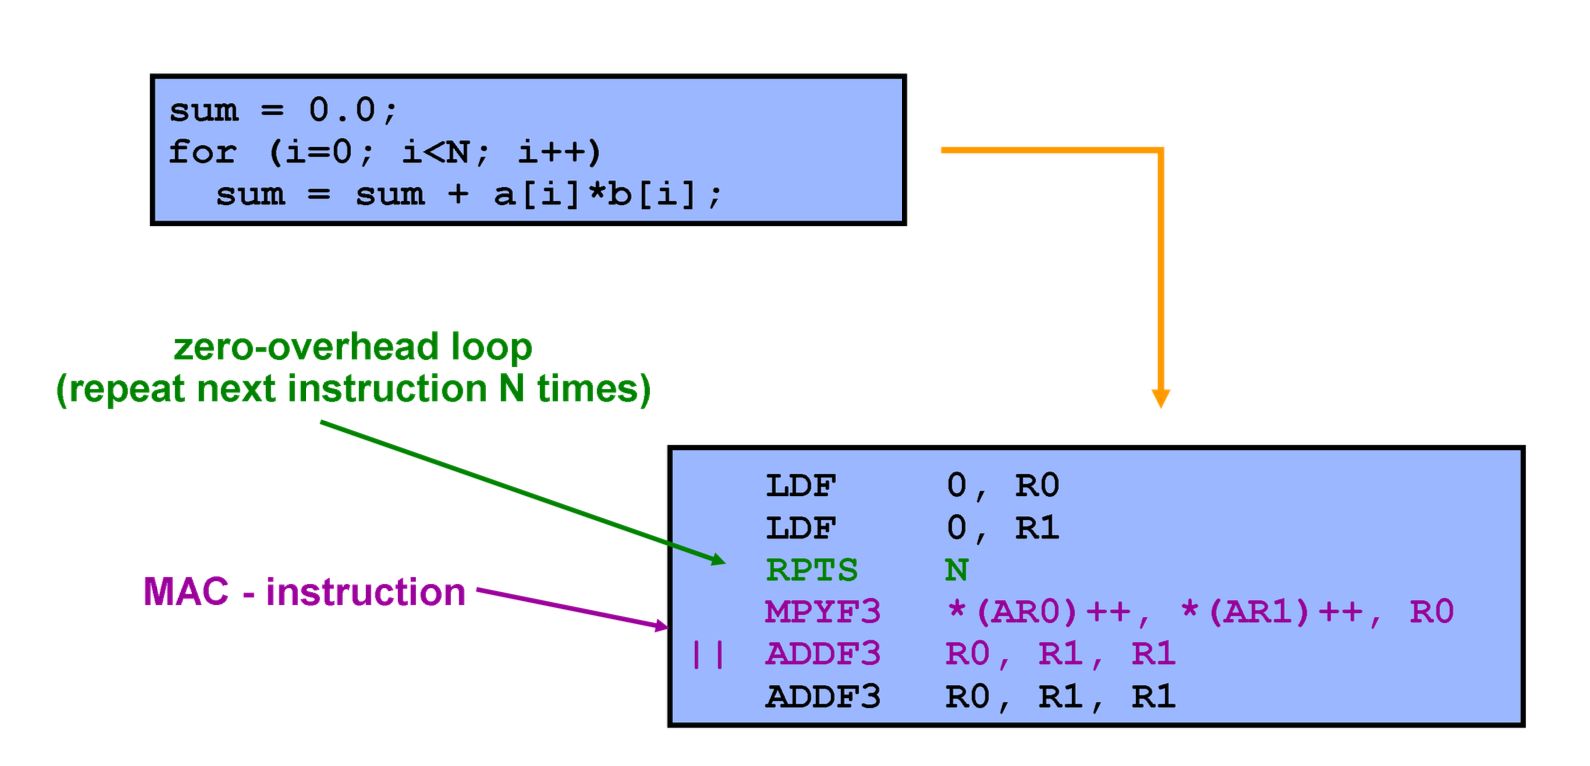
\includegraphics[width=0.5\textwidth]{images/MAC.png}
	\caption{Multiply \& accumulate}
	\label{fig:MAC}
\end{center}
\end{figure}

\subsubsection{DSP - Arithmetics}
\begin{itemize}
	\item Number formats
		\begin{itemize}
			\item Mantissa determines precision
			\item Exponent determines dynamic range
		\end{itemize}
	\item Fixed point
		\begin{itemize}
			\item in case of equal mantissa length smaller (cheaper) and faster as floating-point
			\item application design requires consideration of rounding and scaling problems
			\item sufficient for many DSP applications 
		\end{itemize}
		\item Floating point
		\begin{itemize}
			\item high dynamic range of numbers
			\item easier application program development 
		\end{itemize}
\end{itemize}

\subsubsection{DSP - Program Development}
\begin{itemize}
	\item Assembler, Complier
	\begin{itemize}
		\item Many DSP features still only usable if code is written in assembly
		\item Programming in C $\rightarrow$ profiling $\rightarrow$ time-critical parts in assembly code
	\end{itemize}
	\item Libraries
	\begin{itemize}
		\item Programming in C, call of hand-written optimized functions
	\end{itemize}
	\item Code generation
	\begin{itemize}
		\item Usage of design environments for modeling, simulation and code generation
		\item e.g. Synopsis
	\end{itemize}
\end{itemize}

\subsubsection{DSP - Trends}
\begin{itemize}
	\item Multi-DSP Systems
	\begin{itemize}
		\item for applications requiring highest performance
		\item interfaces available to connect multiple processors
		\item Multi-Processor SoC (MPSoC)
	\end{itemize}
	\item VLIW (Very long instruction word)
	\begin{itemize}
		\item multiple functional units
		\item Compiler detects parallelism and creates a program that schedules multiple instructions jointly
		\item Only useful for applications with high degree of instruction parallelism
		\item suffers often from low code density
		\item compilation difficult
	\end{itemize}
\end{itemize}

\subsection{Application-specific instruction set processors (ASIP)}
\begin{itemize}
	\item Specialization
	\begin{itemize}
		\item instruction set (Operant chaining)
		\item functional units (pixel operations, 1/sqrt(x))
		\item memory architecture (parallel access onto multiple memory banks)
	\end{itemize}
	\item Advantages
	\begin{itemize}
		\item higher performance
		\item lower cost
		\item smaller code images
		\item lower power consumption 
	\end{itemize}
\end{itemize}

\subsection{Integrated Circuit}
\subsubsection{Phases of IC Design}
\begin{enumerate}
	\item Design
	\begin{enumerate}
		\item Modeling
		\item Synthesis \& Optimization
		\item Verification
	\end{enumerate}
	\item Fabrication
	\begin{enumerate}
		\item Masks
		\item Wafer
	\end{enumerate}
	\item Testing
	\item Packaging
	\begin{enumerate}
		\item Slicing
		\item Packaging
	\end{enumerate}	
\end{enumerate}

\subsubsection{Design Styles for ICs}
\begin{figure}[h]
	\begin{center}
		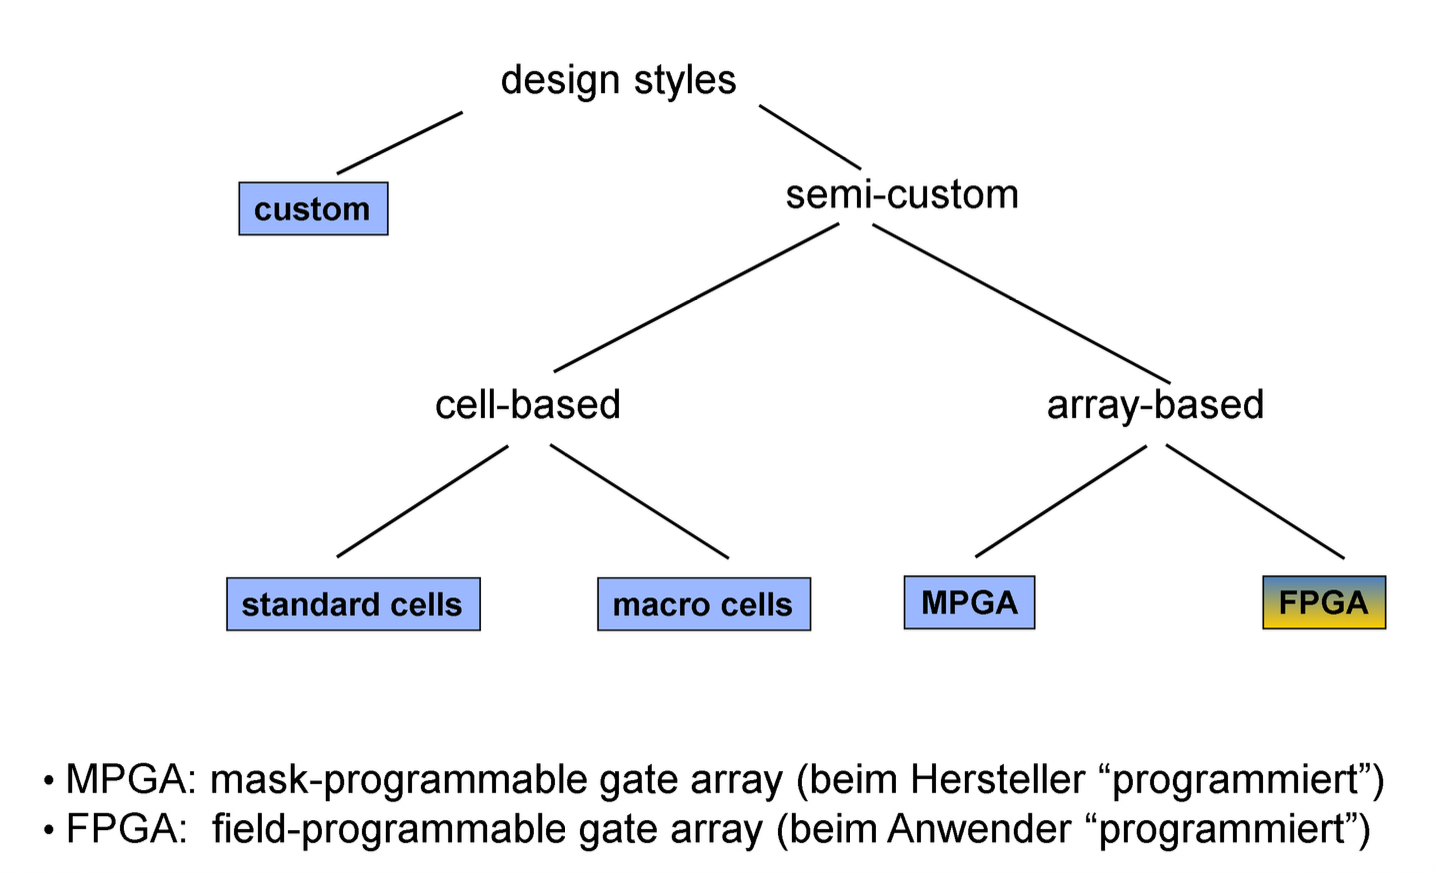
\includegraphics[width=0.5\textwidth]{images/IC_Design_Styles.png}
		\caption{Design Styles for ICs}
		\label{fig:IC_Sty}
	\end{center}
\end{figure}

\subsubsection{Comparison of Design Styles}
\begin{figure}[h]
	\begin{center}
		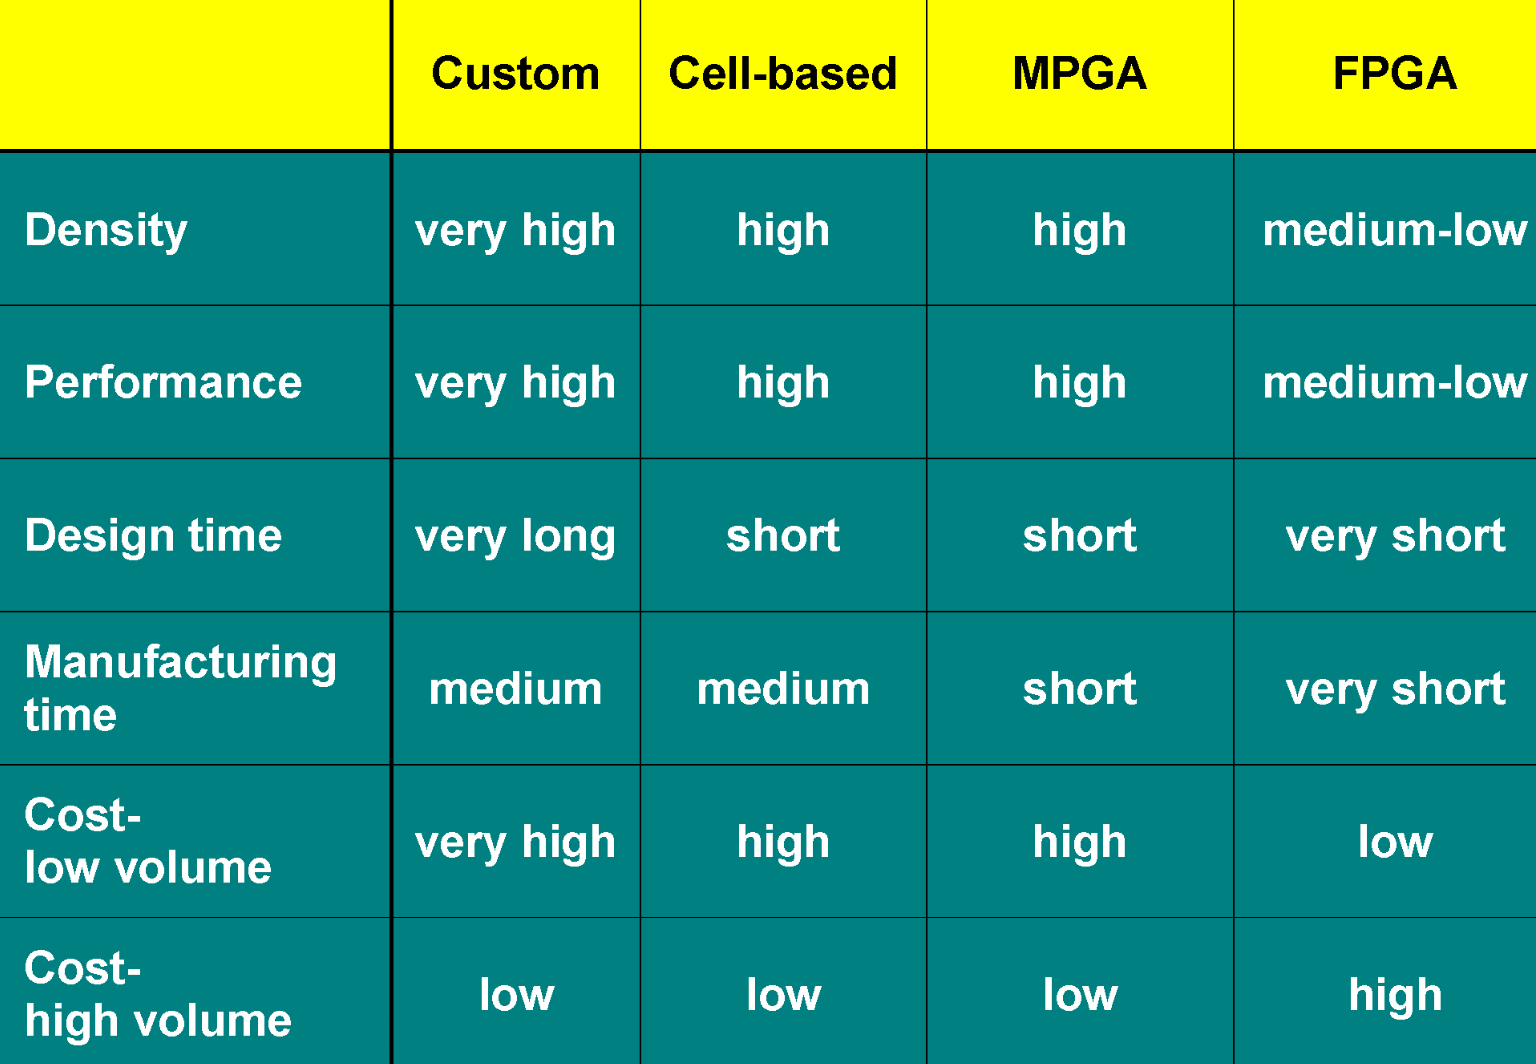
\includegraphics[width=0.5\textwidth]{images/Comp_Des_Sty.png}
		\caption{Comparison of Design Styles}
		\label{fig:Comp_Des_Sty}
	\end{center}
\end{figure}

\subsection{FPGA (field programmable gate arrays)}
\begin{itemize}
	\item Logic blocks
	\item I/O-blocks
	\item Interconnect
\end{itemize}

\subsubsection{FPGA Design Steps}
\begin{figure}[h]
	\begin{center}
		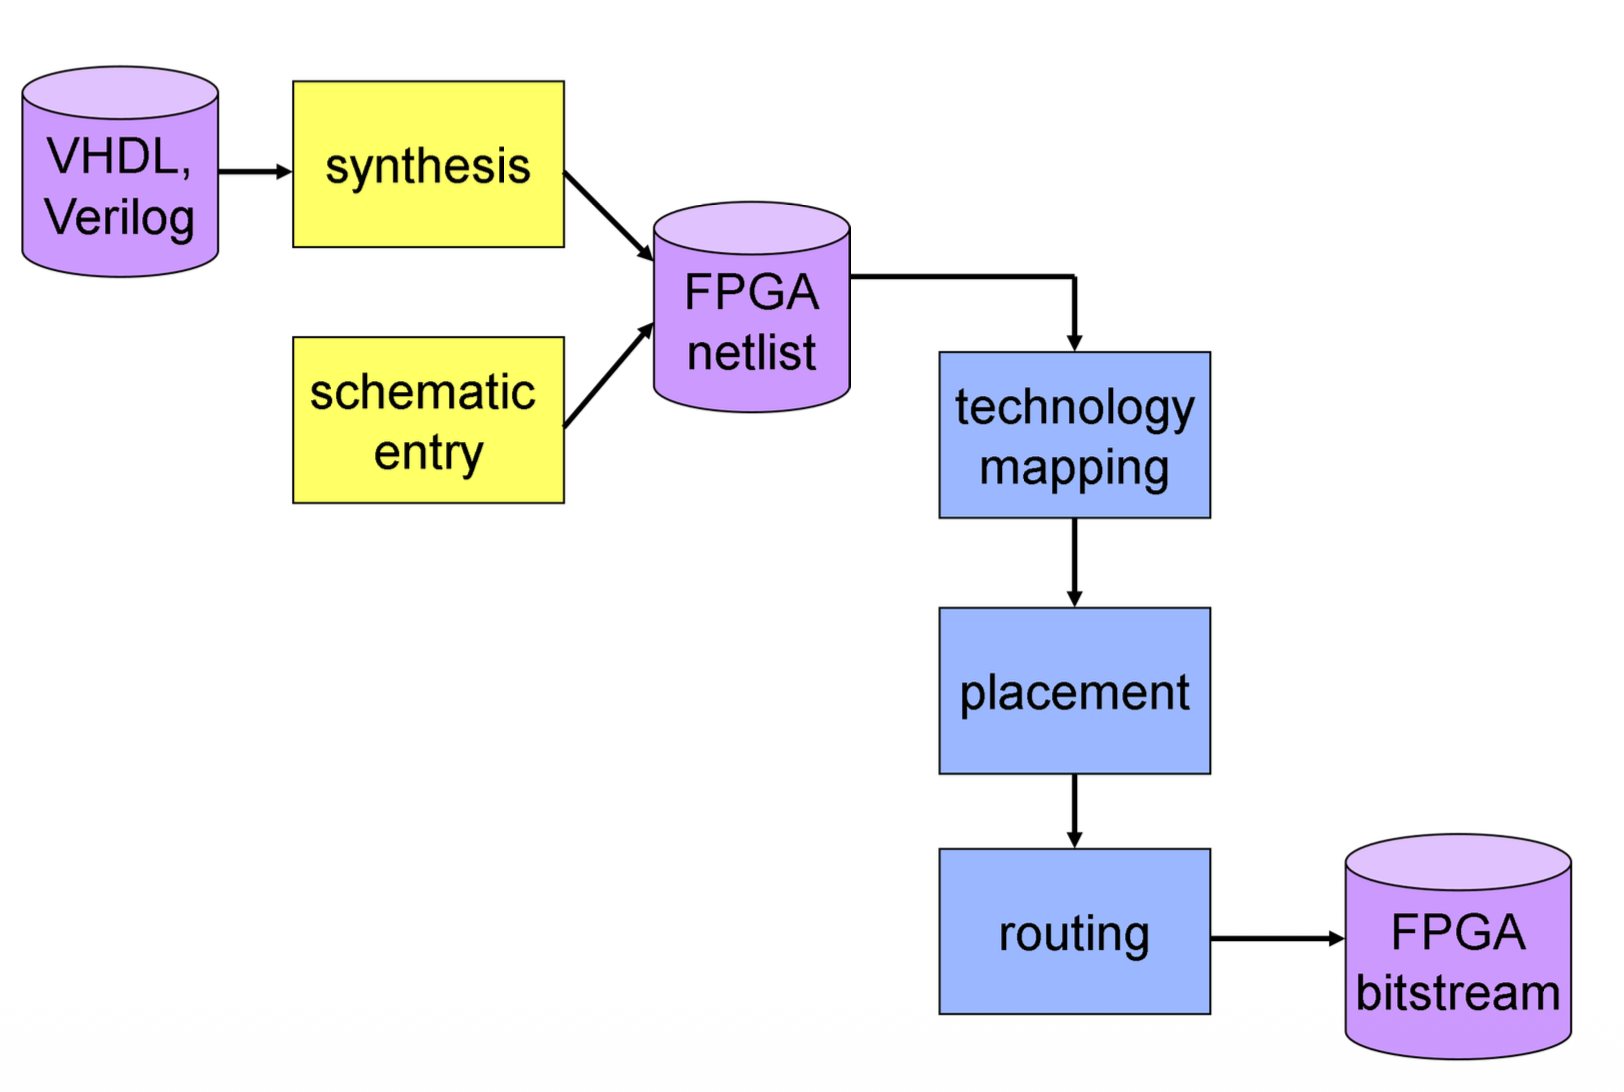
\includegraphics[width=0.5\textwidth]{images/FPGA_Design.png}
		\caption{FPGA design steps}
		\label{fig:FPGA_Des}
	\end{center}
\end{figure}

\subsubsection{FPGA - Application Areas}
\begin{itemize}
	\item Glue Logic
	\item Rapid Prototyping, Emulation
	\item Embedded Systems
	\begin{itemize}
		\item when when processors are too slow or too power-inefficient and
		\begin{itemize}
			\item flexibility is a must
			\item the sale volumes are too low to afford ASIC
		\end{itemize}
	\end{itemize}
	\item Custom Computing
		\begin{itemize}
			\item Goal: Combine flexibility of processors with efficient advantages of ASICs
			\item e.g. Outsourcing a complex task from SW to HW 
		\end{itemize}
\end{itemize}











